\label{sub:SpecO}


Our assertion language %\AssertLang, 
{supports} standard  as well as \emph{object-capability} assertions. 
 The  standard assertions  include the values of fields, implication, quantification etc, as well as ghost fields; the latter can represent user-defined predicates. 
The  object capability assertions express restrictions of an object's eventual authority on some other object.

\begin{definition}
\label{def:assert:syntax}
Expressions, $\re$, and assertions, $A$,  are defined as follows:

\label{f:chainmail-syntax}
$
\begin{syntax}
\syntaxElement{\re}{}
		{
		\syntaxline
				{\prg{true}}
                                {{\alpha}}
				{{x}}
                                {\re.f}
				{\re.f({\overline{\re}})}
		\endsyntaxline
		}
\endSyntaxElement

\syntaxElement{A}{}
		{
		\syntaxline
				{{\re}}
				{{\re} : C}
				{\neg A}
				{A\ \wedge\ A}
				{\all{x:C}{A}}
				{\external{{\re}}}
 				{\protectedFrom{{\re}} {{\re}}} 
				 {\inside {{\re}}} 
		\endsyntaxline
		}
\endSyntaxElement\\
\end{syntax}
$
%In the above, we expect that
\footnote{Addresses in assertions % may contain addresses; 
as \eg  in  $\alpha.blnce > 700$, %. While addresses make little sense in user-written assertions, they are 
are useful when giving semantics to universal quantifiers 
\cf Def. \ref{def:chainmail-semantics}.(\ref{quant1}), {when the local map changes \eg upon call and return, and in general,} for scoped invariants, \cf Def. \ref{def:necessity-semantics}.}

\vspace{.1cm}

{$\fv(A)$ returns the free variables in $A$; for example, $\fv(a\!:\!Account \wedge \forall b:int.[a.\balance = b])$=$\{ a \}$.} 
% {{Moreover, $\fv(A)$ is defined in the obvious way to to return   the free variables in $A$; for example, $\fv(a\!:\!Account \wedge \forall b:int.[a.\balance = b])$=$\{ a \}$.}}
Here 
$f$ stands  for a field, or a ghost  field, but not a method -- \ie no
side-effects.\footnote{The syntax does  not distinguish between fields and ghost fields.
\Eg  $\prg{a}.\prg{\balance}$ may, in some modules (\eg in \ModA), be a field lookup, while in others (e.g. when  balance is defined though an entry in a lookup table) may execute %executing 
a ghost function. 
}
\end{definition}

\forget{
\noindent
\textbf{NOTES}  \notesep % Extended expressions, $\re$, and therefore also 
 Assertions  may contain addresses; \eg   $\alpha.bal > 700$. 
{While addresses make little sense in user-written assertions, they are useful when giving semantics to universal quantifiers 
\cf Def. \ref{def:chainmail-semantics}.(\ref{quant1}), {when the local map changes \eg upon call and return, and in general,} for two-state invariants, \cf Def. \ref{def:necessity-semantics}.(2).}
\notesep The syntax does  not distinguish between fields and ghost fields. For instance, $\prg{a}.\prg{\balance}$ may, in some modules (\eg in \ModA), be a field lookup, while in others (e.g. when the balance is defined though an entry in a lookup table) may involve executing a ghost function. 
% -  $\external {\re}$ is short for $\neg \internal {\re}$. We use these forms freely in the subsequent text without further definition.
%\kjx{These NOTES seem to make heavy work of mostly trivial points
%{{SD: WIll work on that}}
% \footnoteSD{{\textbf{NOTE for us} It also allows assertions like $a1.passwd \neq a2.passwd$, whereas in the past we would have written as $\exists x,y.[\ a1.passwd=x \wedge  a2.passwd=y \wedge x\neq y\ ]$.}} \footnoteSD{{TODO compare with oopsla }}
}


\begin{definition}[Shorthands] 
{We write $\internal{\re}$ for $\neg (\external {\re})$}, and
$\extThis$. resp. {$\intThis$} for $\external{\prg{this}}$ resp. $\internal{\prg{this}}$. %, and $\re:\prg{intl}$ as short for $ \neg \external {\re}}$. 
Forms as $A \rightarrow A'$,  $A \vee A'$, and $\exists x:C.A$  can be encoded.
%; we use these forms freely in the subsequent text.
% without further definition.
\end{definition}



%\begin{definition}[Satisfaction  of Assertions by module and  state] 
\label{def:chainmail-semantics-all}
\label{def:chainmail-semantics}
Satisfaction  of Assertions by module and  state is expressed through  through \ \ $\satisfiesA{M}{\sigma}{{A}}$ \ \ \ and defined by cases on the shape of $A$, in definitions \ref{def:chainmail-semantics}, \ref{def:chainmail-protection-from}, and 
 \ref{def:chainmail-protection}.
%\end{definition}

\footnoteSD{say why we split the def into three defs.} 
\noindent
%\textbf{NOTE}  
Note that while execution takes place in the context of one or more modules, $\Mtwo$, satisfaction of assertions considers \emph{exactly one} module  $M$ -- the internal module. 
%{This is not surprising since the goal of this work is to ensure that external modules cannot break our (internal) module's assertions.}
%\footnoteSD{We need to have clarified internal module earlier.} 
%In most cases, satisfaction depends only on the state $\sigma$, but 
% in some cases it also depends on the module $M$: namely execution of extended expressions   
{$M$} is used % might need to 
 to look up the definitions of ghost fields, and to find class definitions to determine whether an object is  external.
% -- c.f. Def. \ref{def:chainmail-semantics}, cases (\ref{cExpr}),  (\ref{cInternal}). %,  and (\ref{cExternal}) .

\subsection{Semantics of assertions % \AssertLang 
-- first part}
\label{sect:semantics:assert:standard}

% An illustration of the concept of reachable appears in the next subsection, in Fig. \ref{fig:Relevant}.
To determine satisfaction of an expression, we    use the evaluation relation, $\eval{M}{\sigma}{e}{v}$,
which says that the expression $e$ evaluates
to value $v$ in the context of state $\sigma$ and module $M$.
As expressions in \LangOO may be recursively defined, their evaluation 
need not   % may not necessarily 
 terminate. Nevertheless, the logic of $A$ remains classical because recursion is restricted
to expressions, and not generally to assertions.
\footnoteSD{
The semantics of $\hookrightarrow$ {is} unsurprising 
(see {the appendices %of the full paper 
\cite{necessityFull}).}
We have taken this approach from \citeasnoun{FASE}, which also contains a mechanized Coq proof that assertions are classical \cite{coqFASE}. } %Fig.\ref{f:evaluation}).


\begin{definition}[Satisfaction 
of Assertions -- first part] 
\label{def:chainmail-semantics}
We define satisfaction of an assertion $A$ by a % program 
state $\sigma$ with 
 module $M$ as:
\begin{enumerate}
\item
\label{cExpr}
$\satisfiesA{M}{\sigma}{{\re}}\ \ \ \triangleq \ \ \   \eval{M}{\sigma}{{\re}}{\true}$
\item
\label{cClass}
$\satisfiesA{M}{\sigma}{{{\re}} : C}\ \ \ \triangleq \ \ \   \eval{M}{\sigma}{{\re}}{\alpha}\   \wedge \ \class{\alpha} {\sigma}= C$
\item
$\satisfiesA{M}{\sigma}{\neg A}\ \ \ \triangleq \ \ \   {M},{\sigma}\not\models{A}$
\item
$\satisfiesA{M}{\sigma}{A_1\ \wedge\ A_2}\ \ \ \triangleq \ \ \   \satisfiesA{M}{\sigma}{A_1} \   \wedge \ \satisfiesA{M}{\sigma}{A_2}$
%\item
%$\satisfiesA{M}{\sigma}{A_1\ \vee\ A_2}\ \ \ \triangleq \ \ \   \satisfiesA{M}{\sigma}{A_1}\   \vee \ \satisfiesA{M}{\sigma}{A_2}$

\item
\label{quant1}
$\satisfiesA{M}{\sigma}{\all{x:C}{A}} \ \ \ \triangleq \ \ \   
\forall \alpha.[\   \satisfiesA {M}{\sigma} {\alpha:C}  \ \Longrightarrow   \ \satisfiesA{M}{\sigma} {A[\alpha/x]} \ ] $

%\item
%\label{quant2}
%$\satisfiesA{M}{\sigma}{\ex{x:C}{A}}$ \ \ \ iff \ \ \  
% {$\exists \alpha.[\ \GRelevant \alpha \sigma \wedge  \satisfiesA {M}{\sigma} {\alpha:C}  \ \wedge \ \satisfiesA{M}{\sigma} {A[x/\alpha]}\ ]$.} 
%\item
%\label{cInternal}
%$\satisfiesA{M}{\sigma}{\internal{{\re}}}$ \ \ \ iff \ \ \   $\satisfiesA{M}{\sigma}{{{\re}} : C} \ \wedge\ \ C \in M$
\item
\label{cExternal}
$\satisfiesA{M}{\sigma}{\external{{\re}}} \ \ \ \triangleq \ \ \  \exists C.[\ \satisfiesA{M}{\sigma}{{{\re}} : C} \ \wedge \ C \notin M \ ]$
\end{enumerate}
\end{definition}

 
Note that while execution takes place in the context of one or more modules, $\Mtwo$, satisfaction of assertions considers \emph{exactly one} module  $M$ -- the internal module. 
{$M$} is used  mto look up the definitions of ghost fields, and to % find class definitions to 
 determine whether objects are  external.

\subsection{Semantics of Assertions - second part}  

\label{sect:protect}
      
\sdN{In the object capabilities model \cite{MillerPhD}, \emph{permission} 
-- i.e.,  access to a capability -- is a necessary precondition  for producing a given effect;  encapsulated by the principle that "authority (to cause an effect) implies eventual permission" \cite{permissionAuthority}.
As   in \S \ref{sec:shop}, and also \cite{OOPSLA22}, if no external object holds eventual permission for a given capability, then the corresponding effect cannot occur.
 Specifically,  we say that $o$ \emph{has eventual permission to} $o'$, to mean  that $o$ either currently has or will acquire direct access to $o'$ in the future \cite{permissionAuthority}.
}

\sdN{
Given this, it becomes essential to devise methods to determine whether eventual permission exists in a given state. 
Unfortunately, this determination is undecidable, as it depends not only on the current object graph but also on the program code being executed.

In this work, we over-approximate lack of eventual permission through a combination of two properties: one pertaining to the state, and the other to the internal code. 
The state-related property is that   $o$ is \emph{protected} if, on any path from a locally reachable object to $o$, the penultimate object  is internal. 
The program-related property is that it preserves the protection of object $o$.
}

\sdN{
It is straightforward to see that if $o$ is protected and the internal code preserves its protection, then no external object can gain eventual permission to $o$.
We now define "protected":
}
%\citet{OOPSLA22} develop the contrapositive: ``lack of eventualpermission to the relevant capability implies that the given effect will {not} take place''.

%A precise characterization of eventual permission is undecidable, but we approximate it through the concept of \textbf{\emph{protection}}:
%{An object $o$ is \emph{protected  from} another object $o'$, if $o'$ can obtain direct access to   $o$ only if 
%$o$ is \emph{introduced} to some external object $o_e$ by some internal object $o_i$ -- where $o'$ and $o_e$, and also $o$ and $o_i$ may be different.  
%We  use ``introduce'' following \citet{MillerPhD}, where $o$ is is ``introduced'' to $o'$ by $o''$, iff either $o''$ sends to $o'$ a message containing $o$, 
%or $o'$ calls $o''$, and $o''$ eventually returns  $o$ as the result of that call.}
% 
%We now introduce % the concept of 
%(absolute) protection.
%An object is protected, if it is protected from all locally reachable {external} objects. This can also be understood as 
%``protected from the top frame''. \footnoteSD{TODO: motivate; many external objects, no matter which one has unprotected access to an object }

\begin{definition}[Satisfaction 
of Assertions  -- Protection] 
\label{def:chainmail-protection-from}
\label{sect:semantics:assert:prtFrom}
 \label{def:chainmail-protection}
-- continuing definitions in \ref{def:chainmail-semantics}:
\begin{enumerate}
\item
\label{cProtected}
 $\satisfiesA{M}{\sigma}{\protectedFrom{{\alpha}} {{\alpha_{o}}}}   \ \ \ \triangleq $ 
  \begin{enumerate}
 \item
$\alpha\neq \alpha_0$,
 \ \ \ \  and% \\
 \item
$\forall n\in\mathbb{N}. \forall f_1,...f_n..
[\ \ \interpret{\sigma}{\alpha_{o}.f_1...f_n}=\alpha \ \ \  \Longrightarrow \ \ \  \satisfiesA{M}{\sigma}{ {\interpret{\sigma}{\alpha_{o}.f_1...f_{n-1}}}:C} \ \wedge \ C\in M\ \ ]$
\end{enumerate}
\item
$\satisfiesA{M}{\sigma}{\protectedFrom{{\re}} {{\re_{o}}}} \ \ \ \triangleq 
% $ \\ $ 
\ \ \ \exists \alpha, \alpha_{o}. [\  \ \eval{M}{\sigma}{{\re}}{\alpha}\ \wedge \eval{M}{\sigma}{{\re_0}}{\alpha_0} \  \wedge \ 
  \satisfiesA{M}{\sigma}{\protectedFrom{{\alpha}} {{\alpha_{o}}}}
 \ \  ]$
\item
\label{sect:semantics:assert:prt}
$\satisfiesA{M}{\sigma} {\inside {\re}}  \ \ \ \ \triangleq $ 
\begin{enumerate}
\item
{$\forall \alpha.[\ \alpha \in \LRelevantO   {\sigma}\ \wedge\ { \satisfiesA{M}{\sigma}{\external \alpha}} \ \ \Longrightarrow \ \  \satisfiesA{M}{\sigma}{\protectedFrom{\re} {{\alpha}}}\ ] $}, \ \ \ and 
\item
$\satisfiesA{M}{\sigma}{\extThis}\ \ \Longrightarrow\ \ \forall x\!\in\! \sigma.\ \satisfiesA{M}{\sigma}{x\neq \re}$
\end{enumerate}
\end{enumerate}
 \end{definition} 
 

% \vspace{.5cm}
\footnoteSD{JAMES' comment: If is possible that "we" do not know the complete heap (eg we only know about the green stuff.) how do we know whether an object is protected. The answer is that we do not know that it is protected, but we do know that our code guarnartees poreservation of protectedness.
%Nevertheless, if the objects are "robust" then we can prove that some properties will be preserved. 
}
\footnoteSD{
OLD COMMENTS: ${\inside {\_}}$  is central to thinking about capabilities. For example, the balance of an account whose
  password is  encapsulated/protected?  will not decrease in the next step.
  Often, API implementations contain objects whose capabilities, while  crucial for the implementation, if exposed,
would break the intended guarantees of the API. Such objects need to remain confined - see
such an example in Section \ref{s:examples}. 
}
\footnoteSD{{\textbf{TODO} make the connection with domination}}
\footnoteSD{SD Can we think of a better name than protection? \kjx{encapsulation}{No, encapsulation not good}}

Figure \ref{fig:ProtectedFrom} illustrates "protected from" and "protected". % protection from other objects. 
Pink and green indicate external and internal objects respectively.
\sd{In the first row  we  highlight in yellow} the objects protected from other objects. Thus, all objects except $o_6$ are protected from $o_5$ (left pane);\ all objects expect $o_8$ are protected from $o_7$ (middle pane);\ and all objects except $o_3$, $o_6$, $o_7$, and $o_8$ are protected from $o_2$ (right pane). 


\begin{figure}[tbh]
\begin{tabular}{|c|c|c|}
\hline  
\resizebox{4.5cm}{!}{
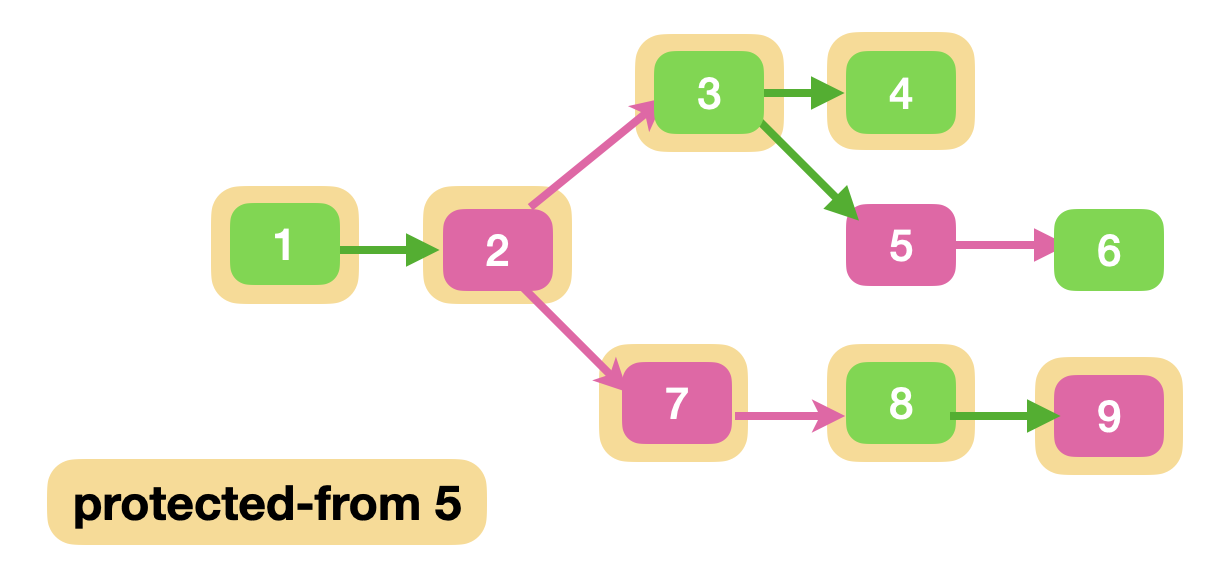
\includegraphics[width=\linewidth]{diagrams/prfA.png}
} 
&
\resizebox{4.5cm}{!}{
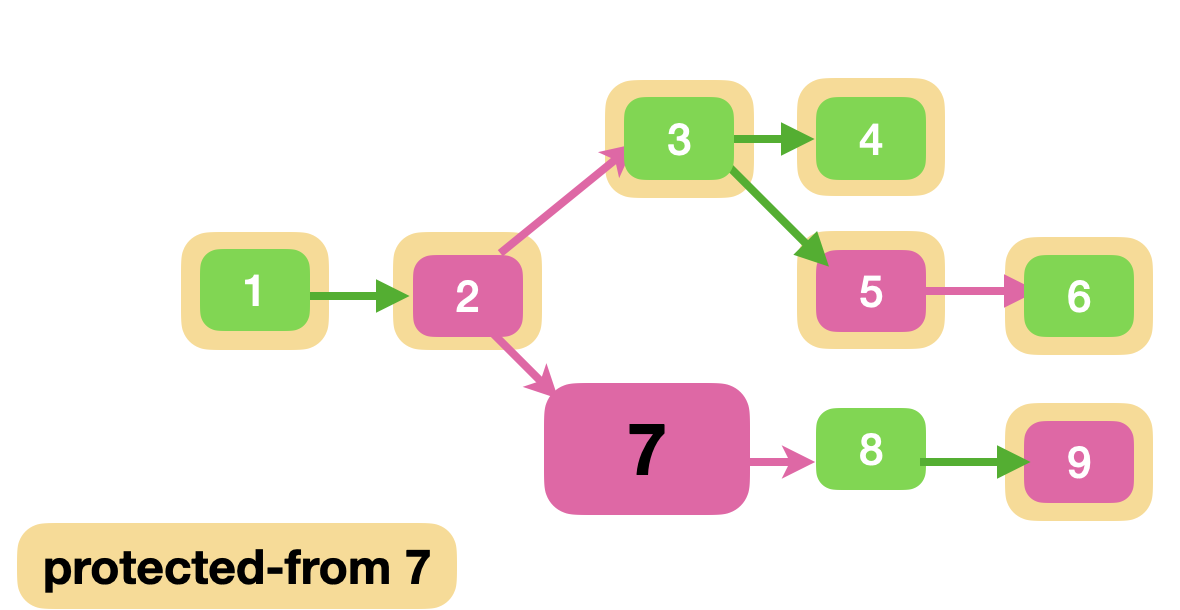
\includegraphics[width=\linewidth]{diagrams/prfB.png}
} 
&
\resizebox{4.5cm}{!}{
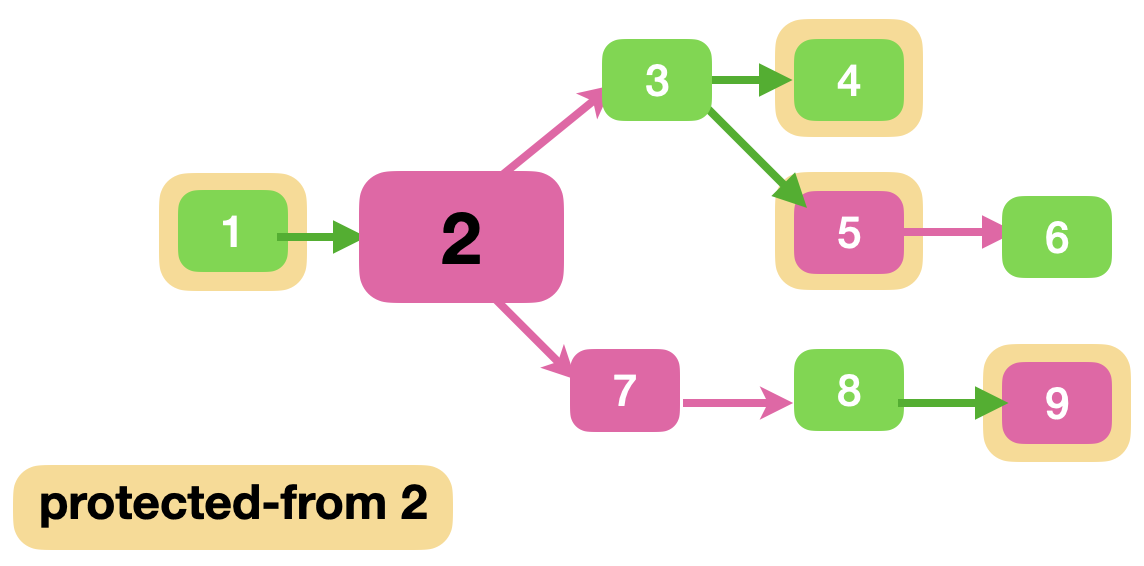
\includegraphics[width=\linewidth]{diagrams/prfC.png}
} 
\\
\hline
protected from $o_5$
&
protected from $o_7$
&
protected from $o_2$
\\
\hline  \hline
\resizebox{4.5cm}{!}{
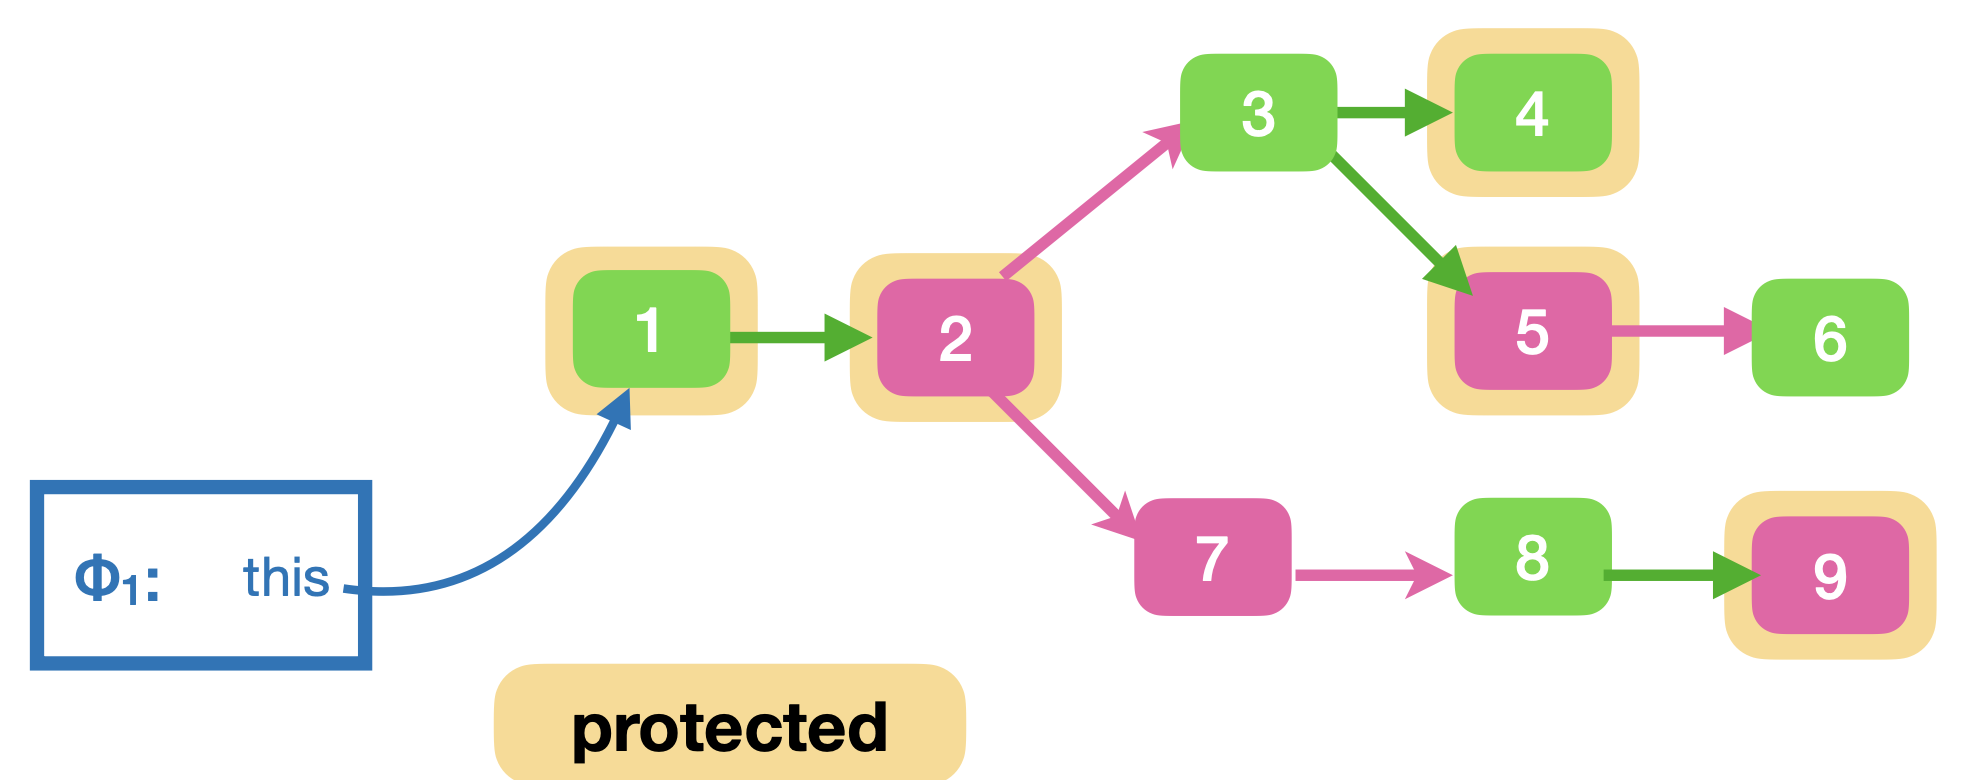
\includegraphics[width=\linewidth]{diagrams/prtFirst.png}
} 
&
\resizebox{4.5cm}{!}{
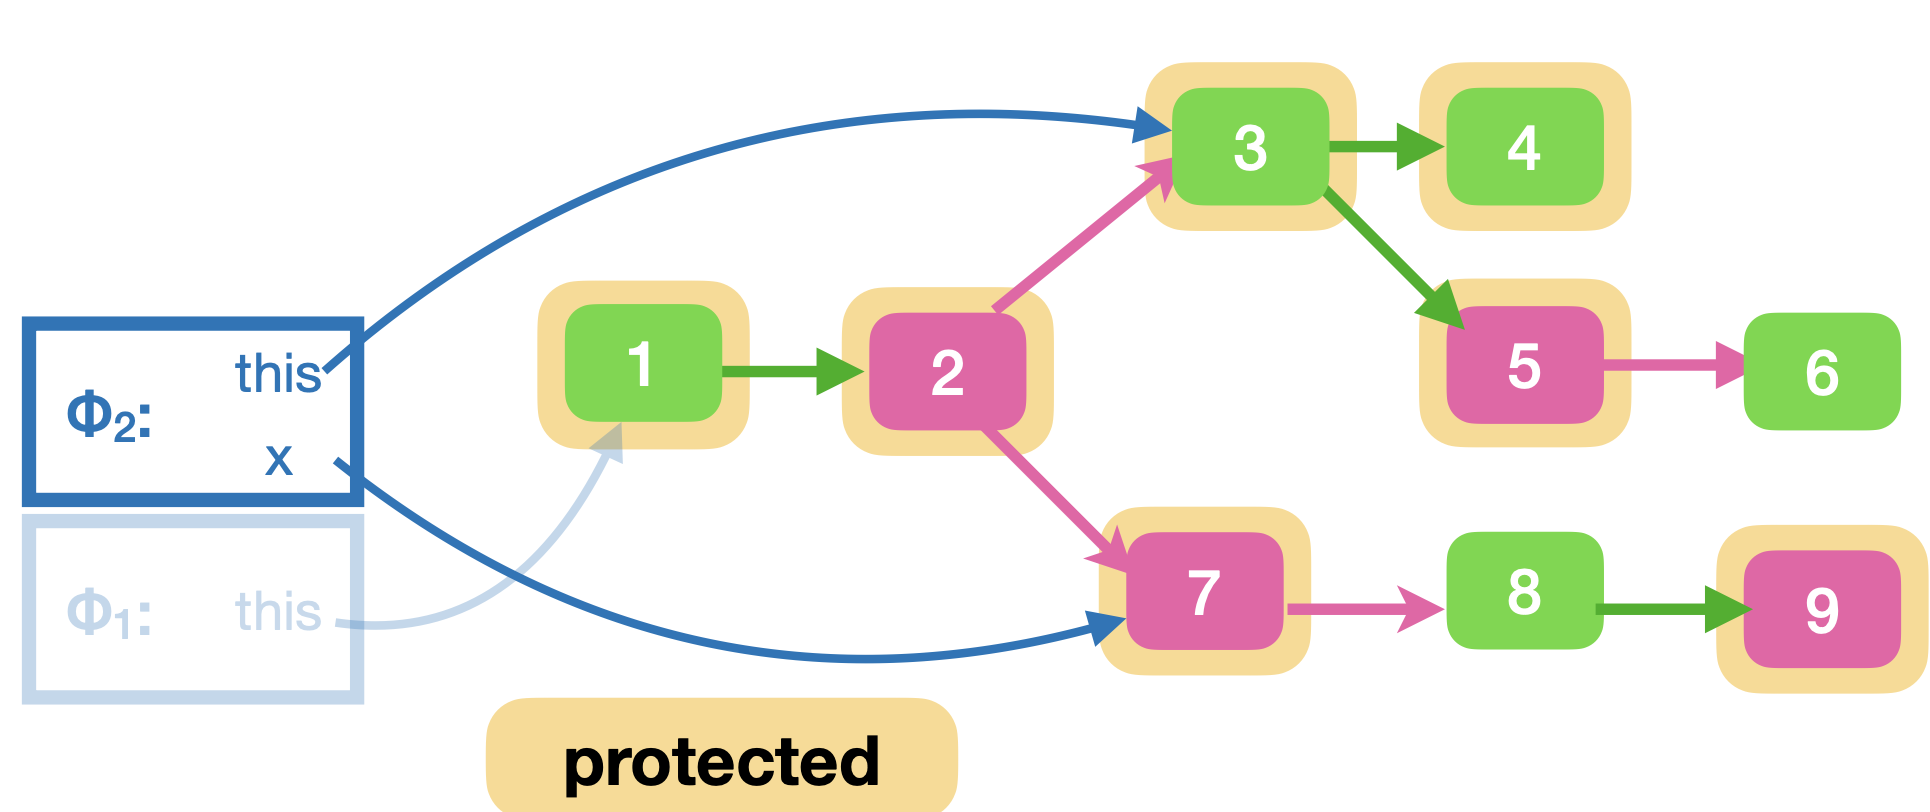
\includegraphics[width=\linewidth]{diagrams/prtSecond.png}
} 
&
\resizebox{4.5cm}{!}{
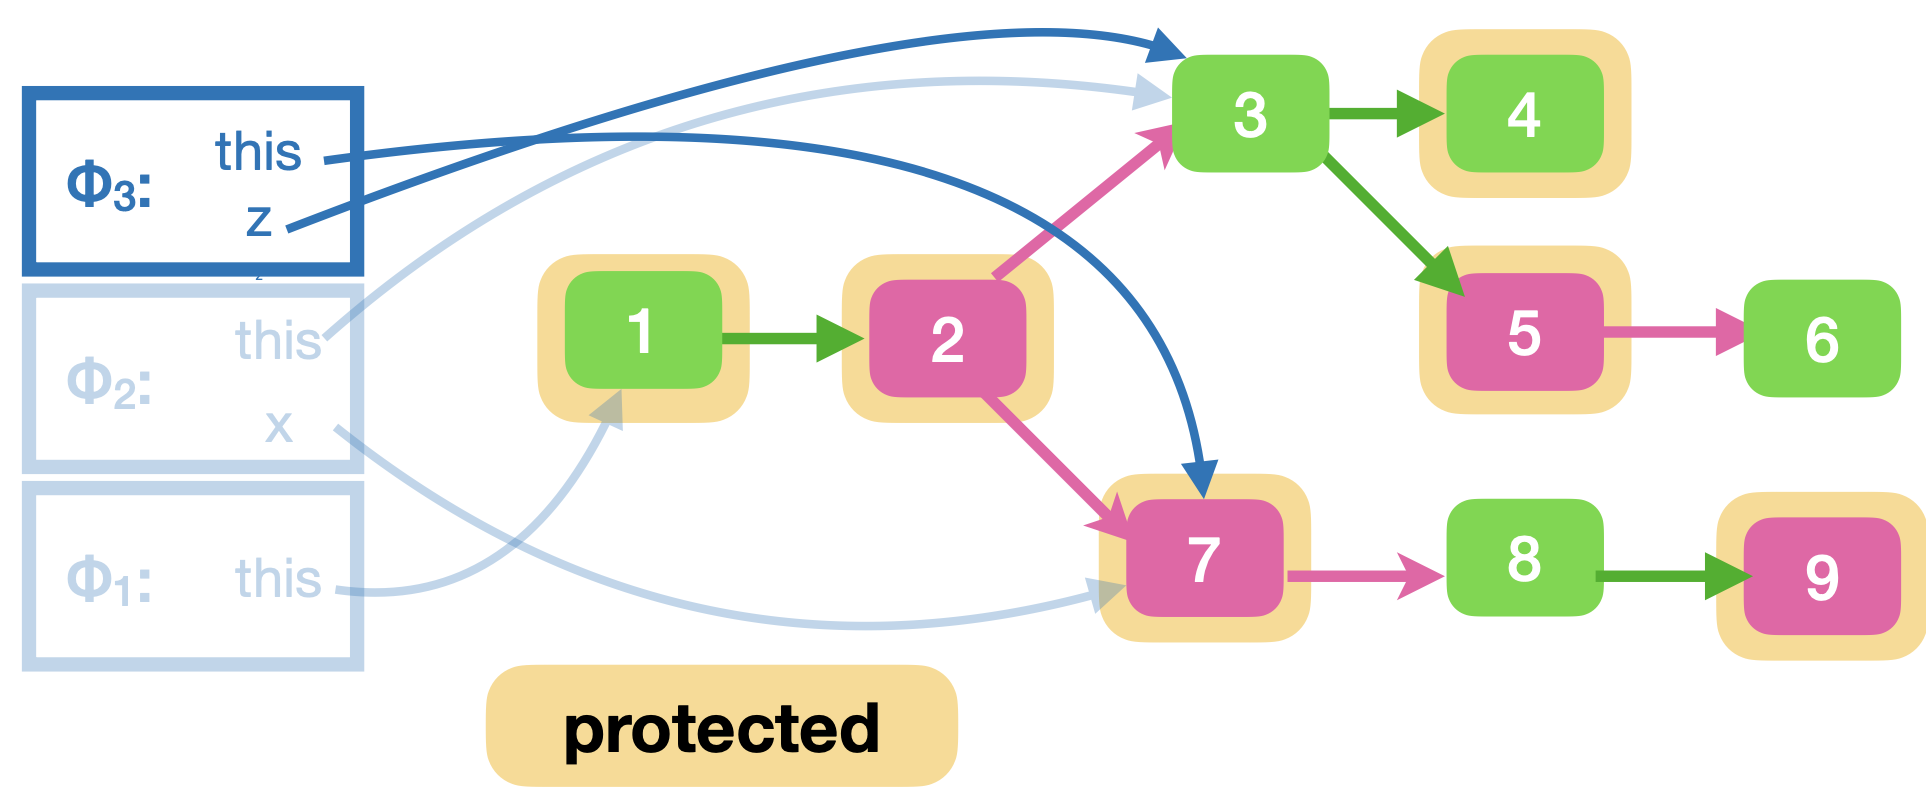
\includegraphics[width=\linewidth]{diagrams/prtLast.png}
} 
\\
\hline
protected in $\sigma_1$ & % with top frame $\phi_1$ &
protected   in $\sigma_2$ & % with top frame $\phi_2$ &
protected  in $\sigma_3$  % with top frame $\phi_2$ &
\\
\hline \hline
\end{tabular}
   \caption{ Protection. Pink objects are external, and green objects are internal.}
   \label{fig:ProtectedFrom}
    \label{fig:Protected}
 \end{figure}
 
 

%Note that $o_8$ is not protected from $o_2$ because there is a path from $o_2$ to $0_8$ which only traverses external objects. Note also, that even though $o_9$ is external, it is protected from $o_7$.
Note that $o_6$ is not protected from $o_2$. 
Namely, even through there are some internal objects on the path from $o_2$ to $o_6$, in our current model, these objects are not sufficient to prevent eventual, unmitigated access of $o_2$ to $o_6$: it is possible for $o_2$ to make a call to $o_3$, and then this call to return $o_5$. Once $o_2$ has access to $o_5$, it can also get access to $o_6$. 

% \vspace{.1in}

%We now introduce % the concept of 
%(absolute) protection.
%An object is protected, if it is protected from all locally reachable {external} objects. This can also be understood as 
%``protected from the top frame''. \footnoteSD{TODO: motivate; many external objects, no matter which one has unprotected access to an object }
 
%\begin{definition}[Satisfaction 
%of Assertions -- Protected] 
%\label{def:chainmail-protection}
%\label{sect:semantics:assert:prt}
%-- continuing definitions from \ref{def:chainmail-semantics} and \ref{def:chainmail-protection-from}:
%\begin{enumerate}
%\item
%$\satisfiesA{M}{\sigma} {\inside {\re}}$  \ \ \ iff \ \ \ 
%\begin{enumerate}
%\item
%{$\forall \alpha.[\ \alpha \in \LRelevantO   {\sigma}\ \wedge\ { \satisfiesA{M}{\sigma}{\external \alpha}} \ \ \Longrightarrow \ \  \satisfiesA{M}{\sigma}{\protectedFrom{\re} {{\alpha}}}\ ] $}, \ \ \ and 
%\item
%$\satisfiesA{M}{\sigma}{\extThis}\ \ \Longrightarrow\ \ \forall x\!\in\! \sigma.\ \satisfiesA{M}{\sigma}{x\neq \re}$
%\end{enumerate}
%\end{enumerate}
%\end{definition} 
 
% TODO explain
In the third row of   Figure \ref{fig:Protected} we show three states: 
% illustrates %the concept of 
%  protection. The heap in all three panes is the same as in  Fig \ref{fig:LReachable} and 
 %Fig \ref{fig:ProtectedFrom}. State  
 $\sigma_1$ has  top frame $\phi_1$, which has  one variable, \prg{this}, pointing to $o_1$, while 
 $\sigma_2$ has  top frame $\phi_2$; it has two  variables,   \prg{this} and \prg{x} pointing to $o_3$ and  $o_7$, and 
 $\sigma_3$ has  top frame $\phi_3$; it has two  variables,  \prg{this} and \prg{x}, pointing to $o_7$ and $o_3$.  
% 
%The locally reachable objects in $\sigma_1$ were highlighted in the middle pane of Fig \ref{fig:LReachable}; 
%the locally reachable objects from $\sigma_2$  are the same as those from $\sigma_3$, and  were  highlighted in the right pane of that
%Fig. 
%In Fig.  \ref{gig:Protected} 
We also   highlight the protected objects with a yellow halo.
 Note that $o_3$ is protected in $\sigma_2$, but is not protected in $\sigma_3$. This is so, because $\interpret {\sigma_3} {\prg{this}}$  is external, and  $o_3$ is an argument to the call. As a result, during the call, $o_7$ may obtain unmitigated access (permission) to $o_3$. 

%\begin{praise}{for protection}
\subsubsection*{Discussion} 
\sdN{Lack of eventual permission is a central concept in the verification of code with calls to and callbacks  from untrusted code.
% ARGHHH a joke citatiion? \cite{praiseYou}.   
%Unmediated access is essentially \citet{MillerPhD}'s permission: that we have a ``first
%class'' reference to the capability; that we can call any 
%method in the capability's public interface; that we can
%store or save or present the capability to any other
%object to which we've been introduced
%%\footnote{``nobody can ever be introduced in a ball-room''}
It has already been over-approximated in several different ways, \eg
2nd-class \cite{rompf-second-class-oopsla2016,rompf-dont-pop-second-class-ecoop2022}
or borrowed (``2nd-hand'') references
\cite{boyland-promises-icse1998,boyland-aliasburying-spe2001},
 textual modules \cite{OOPSLA22},
information flow \cite{ddd}, runtime
checks \cite{secure-io-fstar-popl2024},
abstract data type exports \cite{vmsl-pldi2023},
  separation-based invariants 
Iris \cite{iris-wasm-pldi2023,cerise-jacm2024},
-- more in  \S~\ref{sect:related}.
In general, protection is applicable in more situations (i.e.\ is less
restrictive) than most of these approaches,
 \sdN{although more restrictive than the ideal "lack of eventual permission"}. 
\footnoteSD{ HER WHAT IT USED TO SAY:
the contrapositive ideal that lack of eventual permission ensures
lack of effect. Note that ``cannot get unmitigated access'' does not generally imply ``is
protected''. 
}

It is easy to see that protection and protection preservation are sufficient but not necessary conditions for lack of eventual permission, and that, on the other hand, protection without preservation of protection does not imply lack of eventual permission.
}
%Protection --- \sdN{objects to which external objects may not get %which objects can get 
%unmediated access} % to which other objects 
%---  is  a crucial concept: It enables
%the verification code in the open world, % even in the presence of
%with calls to and callbacks 
%from untrusted code.
%% ARGHHH a joke citatiion? \cite{praiseYou}.   
%Unmediated access is essentially \citet{MillerPhD}'s permission: that we have a ``first
%class'' reference to the capability; that we can call any 
%method in the capability's public interface; that we can
%store or save or present the capability to any other
%object to which we've been introduced
%%\footnote{``nobody can ever be introduced in a ball-room''}
%(compare
%2nd-class \cite{rompf-second-class-oopsla2016,rompf-dont-pop-second-class-ecoop2022}
%or borrowed (``2nd-hand'') references
%\cite{boyland-promises-icse1998,boyland-aliasburying-spe2001}
%which are restricted in some way),
%without reference to some owning class or defining module.
%We discuss alternative designs,
%ranging from overly simplistic textual modules \cite{OOPSLA22},
%information flow \cite{ddd}, runtime
%checks \cite{secure-io-fstar-popl2024},
%abstract data type exports \cite{vmsl-pldi2023},
%to automated separation-based invariants in
%Iris \cite{iris-wasm-pldi2023,cerise-jacm2024},
%in section~\ref{sect:related}.
%In general, protection is applicable in more situations (i.e.\ is less
%restrictive) than most of these approaches,
% \sdN{although more restrictive than the ideal "lack of eventual permission"}. 
%\footnoteSD{ HER WHAT IT USED TO SAY:
%the contrapositive ideal that lack of eventual permission ensures
%lack of effect. Note that ``cannot get unmitigated access'' does not generally imply ``is
%protected''


 
